\documentclass[notes,10pt, aspectratio=169]{beamer}

\usepackage{pgfpages}
% These slides also contain speaker notes. You can print just the slides,
% just the notes, or both, depending on the setting below. Comment out the want
% you want.
\setbeameroption{hide notes} % Only slide
%\setbeameroption{show only notes} % Only notes
%\setbeameroption{show notes on second screen=right} % Both
\usepackage{wrapfig}

\usepackage{helvet}
\usepackage[default]{lato}
\usepackage{array}
\usepackage{eurosym}
\usepackage{setspace}
\usepackage{animate}
\usepackage{multicol}
\usepackage{breqn}
\usepackage{subcaption}
\usepackage{caption}
\captionsetup{font=scriptsize, justification=raggedright,singlelinecheck=false}
\usepackage[export]{adjustbox}
\usepackage[scale=2]{ccicons}
\usepackage{tikz}
\newenvironment{wideitemize}{\itemize\addtolength{\itemsep}{10pt}}{\enditemize}
\usepackage{natbib}

\usepackage{tikz}
\usepackage{verbatim}
\setbeamertemplate{note page}{\pagecolor{yellow!5}\insertnote}
\usepackage{amsmath}
%\usepackage{mathpazo}
\usepackage{hyperref}
\usepackage{lipsum}
\usepackage{multimedia}
\usepackage{multirow}
\usepackage{graphicx}
\usepackage{dcolumn}
\usepackage{bbm}
\newcolumntype{d}[0]{D{.}{.}{5}}

\usepackage{changepage}
\usepackage{appendixnumberbeamer}
% \newcommand{\beginbackup}{
%   \newcounter{framenumbervorappendix}
%   \setcounter{framenumbervorappendix}{\value{framenumber}}
%   \setbeamertemplate{footline}
%   {
%      \leavevmode%
%      \hline
%      box{%
%       \begin{beamercolorbox}[wd=\paperwidth,ht=2.25ex,dp=1ex,right]{footlinecolor}%
% %         \insertframenumber  \hspace*{2ex} 
%       \end{beamercolorbox}}%
%      \vskip0pt%
%   }
%  }
\useinnertheme[shadow]{rounded}
\setbeamercolor{block title example}{fg=black,bg=orange!50!white}
\setbeamercolor{block body example}{fg=black, bg=orange!30!white}
\setbeamercolor{block title}{use=structure,fg=structure.fg,bg=structure.fg!20!bg}
\setbeamercolor{block body}{parent=normal text,use=block title,bg=block title.bg!50!bg}

 \setbeamertemplate{footline}{
    \hbox{%
    \begin{beamercolorbox}[wd=\paperwidth,ht=3ex,dp=1.5ex,leftskip=2ex,rightskip=2ex]{page footer}%
        %\usebeamerfont{title in head/foot}%
        %\insertshorttitle \hfill
        %\insertsection \hfill
        %\tableofcontents[currentsection] \hfill
        \insertsectionnavigationhorizontal{0.7\paperwidth}{}{} \hfill 
        \insertframenumber{} / \inserttotalframenumber
    \end{beamercolorbox}}%
}
\newcommand{\backupend}{
   \addtocounter{framenumbervorappendix}{-\value{framenumber}}
   \addtocounter{framenumber}{\value{framenumbervorappendix}} 
}


\usepackage{graphicx}
\usepackage[space]{grffile}
\usepackage{booktabs}

% These are my colors -- there are many like them, but these ones are mine.
\definecolor{blue}{RGB}{0,114,178}
\definecolor{red}{RGB}{213,94,0}
\definecolor{yellow}{RGB}{240,228,66}
\definecolor{green}{RGB}{0,158,115}

\setbeamercolor{section in head/foot}{fg=blue}


\hypersetup{
  colorlinks=false,
  linkbordercolor = {white},
  linkcolor = {blue}
}


%% I use a beige off white for my background
\definecolor{MyBackground}{RGB}{255,253,218}

%% Uncomment this if you want to change the background color to something else
%\setbeamercolor{background canvas}{bg=MyBackground}

%% Change the bg color to adjust your transition slide background color!
\newenvironment{transitionframe}{
  \setbeamercolor{background canvas}{bg=yellow}
  \begin{frame}}{
    \end{frame}
}

\setbeamercolor{frametitle}{fg=blue}
\setbeamercolor{title}{fg=black}
%\setbeamertemplate{footline}[frame number]
\setbeamertemplate{navigation symbols}{} 
\setbeamertemplate{itemize items}{-}
\setbeamercolor{itemize item}{fg=blue}
\setbeamercolor{itemize subitem}{fg=blue}
\setbeamercolor{enumerate item}{fg=blue}
\setbeamercolor{enumerate subitem}{fg=blue}
\setbeamercolor{button}{bg=white,fg=blue,}



% If you like road maps, rather than having clutter at the top, have a roadmap show up at the end of each section 
% (and after your introduction)
% Uncomment this is if you want the roadmap!
% \AtBeginSection[]
% {
%    \begin{frame}
%        \frametitle{Roadmap of Talk}
%        \tableofcontents[currentsection]
%    \end{frame}
% }

\useinnertheme[shadow]{rounded}
\setbeamercolor{block title example}{fg=black,bg=orange!50!white}
\setbeamercolor{block body example}{fg=black, bg=orange!30!white}
\setbeamercolor{block title}{use=structure,fg=structure.fg,bg=structure.fg!20!bg}
\setbeamercolor{block body}{parent=normal text,use=block title,bg=block title.bg!50!bg}


\setbeamercolor{section in toc}{fg=blue}
\setbeamercolor{subsection in toc}{fg=red}
%\setbeamersize{text margin left=1em,text margin right=1em} 
\setbeamersize{text margin left=0.7cm,text margin right=0.7cm} 


\title[]{\textcolor{blue}{Lecture 4:\\OLS Implementation}}
\author{25117 - Econometrics}
\institute[shortinst]{Universitat Pompeu Fabra}

\date{October 9th, 2024}

\begin{document}



% Title Slide

\begin{frame}[plain]
\maketitle
\end{frame}

\section{Introduction}

\begin{frame}{What we learned in the last lesson}
\begin{itemize}
    \item The population regression line, $\beta_0 + \beta_1 X$, is the mean of $Y$ as a function of the value of $X$.
    \begin{itemize}
        \item The slope, $\beta_1$, is the expected difference in $Y$ between two observations with $X$ values that differ by one unit.
        \item The intercept, $\beta_0$, determines the level (or height) of the regression line.
    \end{itemize}\vspace{1em}
    \item The population regression line can be estimated using sample observations $(Y_i, X_i)$ with $i = 1, \dots, n$ by ordinary least squares (OLS).
    \begin{itemize}
        \item The OLS estimators of the regression intercept and slope are denoted $\hat{\beta}_0$ and $\hat{\beta}_1$.
        \item The predicted value of Y given X is $\hat{Y}=\hat{\beta}_0 + \hat{\beta}_1 X$.
    \end{itemize}\vspace{1em}
\end{itemize}
\end{frame}

\begin{frame}{What we learned in the last lesson}
\begin{itemize}
    \item The $R^2$ and standard error of the regression (SER) are measures of how close the values of $Y_i$ are to the estimated regression line.\\
    \begin{itemize}
        \item The $R^2$ is between 0 and 1, indicating how much variance in our outcome is explained by the variance of our regressors.
        \item The standard error of the regression estimates the standard deviation of the regression error.
    \end{itemize}
    \vspace{1em}
    \item There are three key assumptions for estimating causal effects using the linear regression model:
    \begin{enumerate}
        \item The regression errors, $u_i$, have a mean of 0, conditional on the regressors $X_i$;
        \item the sample observations are i.i.d. random draws from the population; and 
        \item large outliers are unlikely
    \end{enumerate}
    \vspace{1em}
   \item If these assumptions hold, the OLS estimator $\hat{\beta}_1$ is 
    \begin{enumerate}
        \item  an unbiased estimator of the causal effect ${\beta}_1$
        \item consistent
        \item normally distributed when the sample is large.
    \end{enumerate}
\end{itemize}
\end{frame}



\begin{frame}{Estimation of the regression line}
We want to learn about the slope of the population regression line. We have data from a sample, so there is sampling uncertainty. There are five steps toward this goal:
    \begin{enumerate}
        \item State the population of interest 
        \item Provide an estimator of this population object
        \item Derive the sampling distribution of the estimator (this requires certain assumptions). In large samples, this sampling distribution will be normal by the CLT.
        \item The square root of the estimated variance of the sampling distribution is the standard error (SE) of the estimator
        \item Use the SE to construct t-statistics (for hypothesis tests) and confidence intervals.
    \end{enumerate}
\end{frame}


\begin{frame}{Estimation of the regression line}
 \begin{columns}
\begin{column}{0.35\textwidth}
$Y_i = \beta_0 + \beta_1 X_i + u_i$\\\vspace{.5cm}
    \begin{itemize}
        \item $\beta_1$ is the slope of the population regression line
        \item $\hat{\beta}_1$ is the OLS estimator of $\beta_1$
         \item When $n$ is large, by the Central Limit Theorem, the sampling distribution of $\hat{\beta}_1$ is well approximated by a normal distribution $\mathcal{N}(\beta_1; \frac{\sigma^2_u}{TSS_X})$
    \end{itemize}
\end{column}
\begin{column}{0.7\textwidth}
\begin{figure}
  \centering
         \vspace{-5mm}
        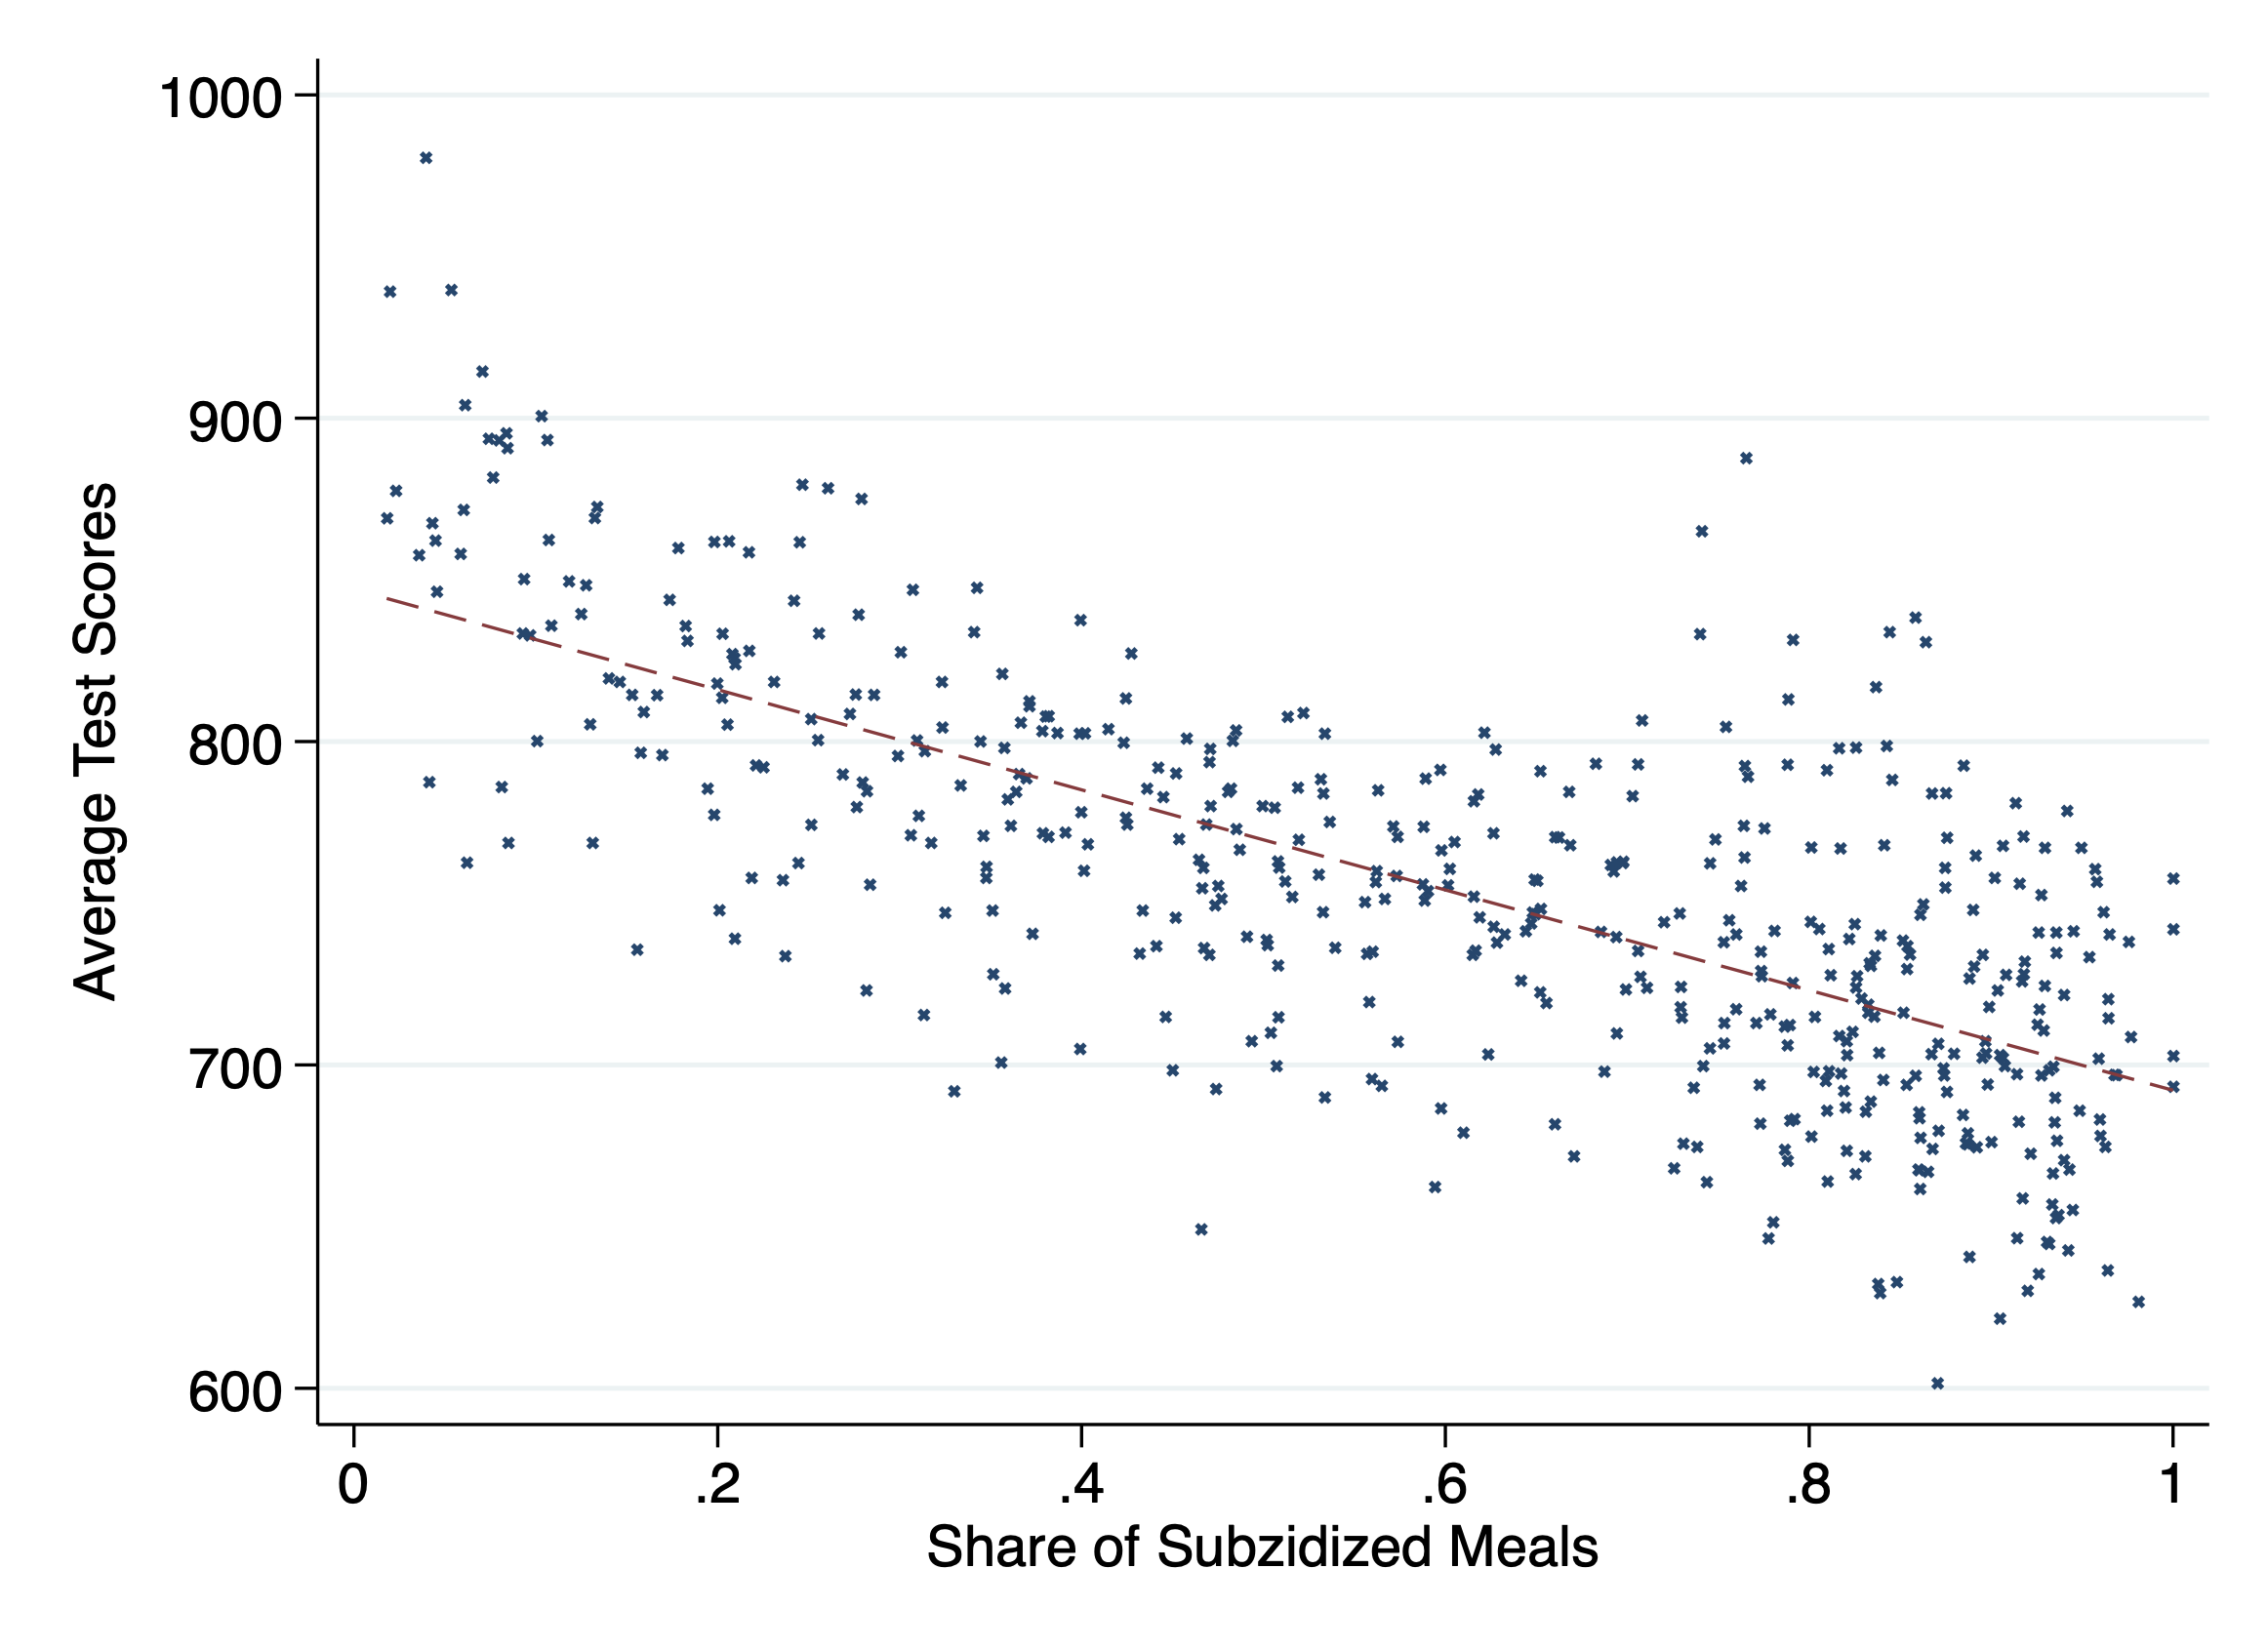
\includegraphics[scale=.25]{images/testscores_corr.png}
\end{figure}
\end{column}
\end{columns}
\end{frame}


\begin{frame}{Hypothesis Testing}
 \begin{columns}
\begin{column}{0.35\textwidth}
    \begin{itemize}
        \item Most of the time, we test for $H_0: \beta_1=0$
        \item Null hypothesis and two-sided alternative:
        \begin{itemize}
            \item $H_0: \beta_1=\beta_{1,0} \text{~~~~vs.~~~~} H_1: \beta_1\neq\beta_{1,0}$ 
        \end{itemize}
        \item Null hypothesis and one-sided alternative:
        \begin{itemize}
            \item $H_0: \beta_1=\beta_{1,0} \text{~~~~vs.~~~~} H_1: \beta_1 < (or >)\beta_{1,0}$ 
        \end{itemize}
    \end{itemize}
\end{column}
\begin{column}{0.7\textwidth}
\begin{figure}
  \centering
         \vspace{-5mm}
        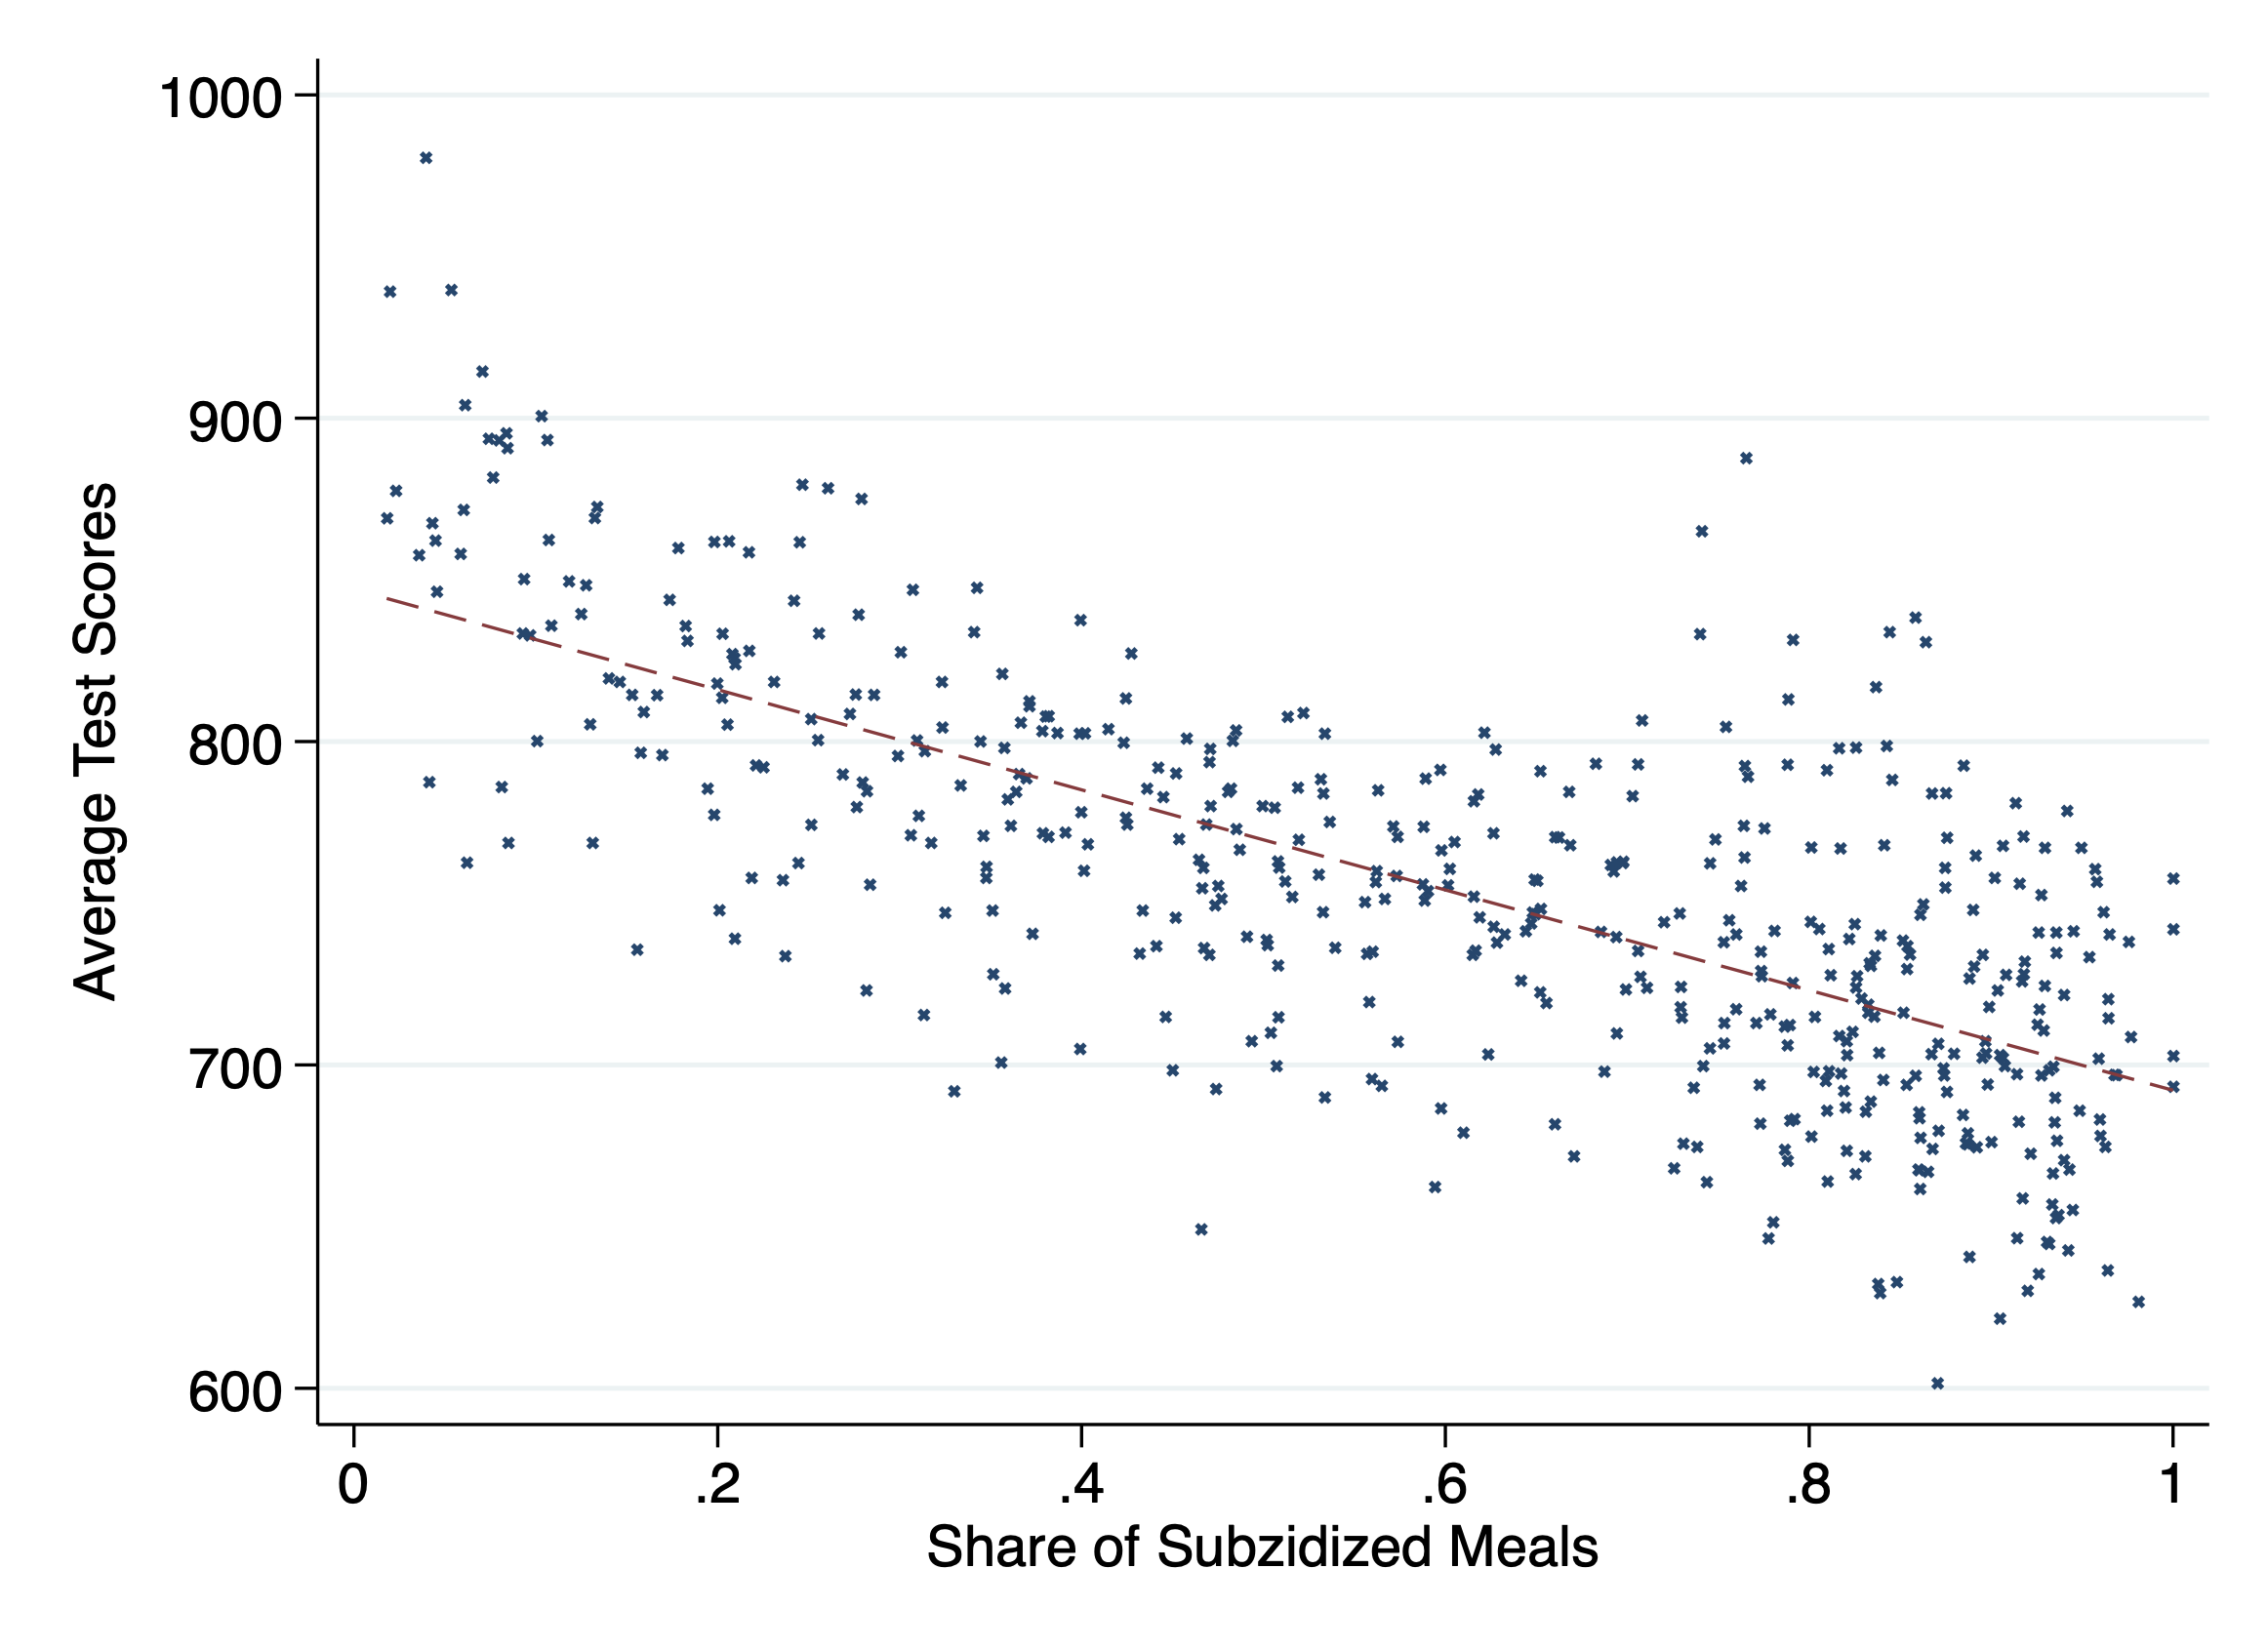
\includegraphics[scale=.25]{images/testscores_corr.png}
\end{figure}
\end{column}
\end{columns}
\end{frame}

\begin{frame}{Hypothesis Testing}
    \begin{itemize}
        \item In general, the t-statistic is given by
        \begin{equation*}
            t=\frac{\text{estimator}-\text{hypothetised value}}{\text{standard error of the estimator}}
        \end{equation*}
        \item For $\mu_{Y}$, the t-statistic is given by
        \begin{equation*}
            t=\frac{\overline{Y}-\mu_{Y,0}}{s_Y/\sqrt{n}}
        \end{equation*}
        \item For $\beta_1$, the t-statistic is given by
        \begin{equation*}
            t=\frac{\hat{\beta}_1-\beta_{1,0}}{SE(\hat{\beta}_1)}
        \end{equation*}
        where $SE(\hat{\beta}_1)=\sqrt{\frac{SSR}{(n-2) TSS_X}}=\sqrt{\frac{\sum_{i=1}^n \hat{u}_i^2}{(n-2)\sum_{i=1}^n (X_i-\overline{X})}}$ when errors are homoskedastic (i.e., $var(u_i\mid X)=\sigma^2_u$~~~$\forall i=1,\dots, n$)
        \item We reject $H_0: \beta_1=\beta_{1,0}$ at 5\% significance level if $\mid t \mid > 1.96$, or alternatively, if $p-value < 0.05$

    \end{itemize}
\end{frame}

\begin{frame}{Stata Application}
 \begin{columns}
\begin{column}{0.3\textwidth}
\begin{itemize}
    \item We regress schools' average test scores ($Y$) against the share of subsidized meals ($X$). 
    \item Our regression sample includes 500 schools ($i=1,\dots, 500$)
\end{itemize}
\end{column}
\begin{column}{0.6\textwidth}
\begin{figure}
  \centering
         \vspace{-5mm}
        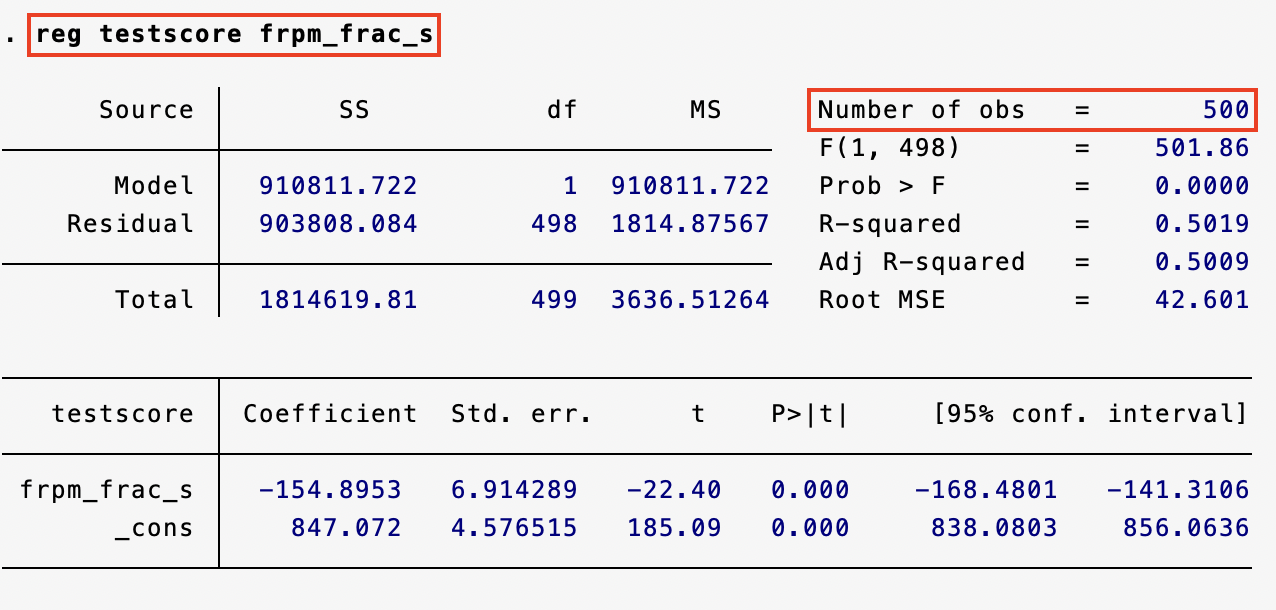
\includegraphics[scale=.4]{images/reg0.png}
\end{figure}
\end{column}
\end{columns}
\begin{center}
\begin{equation*}
    Y_i = \hat{\beta}_0 + \hat{\beta}_1 X_i + \hat{u}_i
\end{equation*}
\end{center}
\end{frame}

\begin{frame}{Stata Application}
 \begin{columns}
\begin{column}{0.3\textwidth}
\begin{itemize}
    \item The estimate of the intercept, $\hat{\beta}_0$ is equal to 847.072
    \item This is the value of the expected average test score for a school not subsidizing meals at all (i.e., $X_i = 0$)
    \item Because all schools in our sample data subsidize a non-zero share of meals, it does not really have a real-world interpretation
    %\item It is the coefficient that determines the level of the regression line
\end{itemize}
\end{column}
\begin{column}{0.6\textwidth}
\begin{figure}
  \centering
         \vspace{-5mm}
        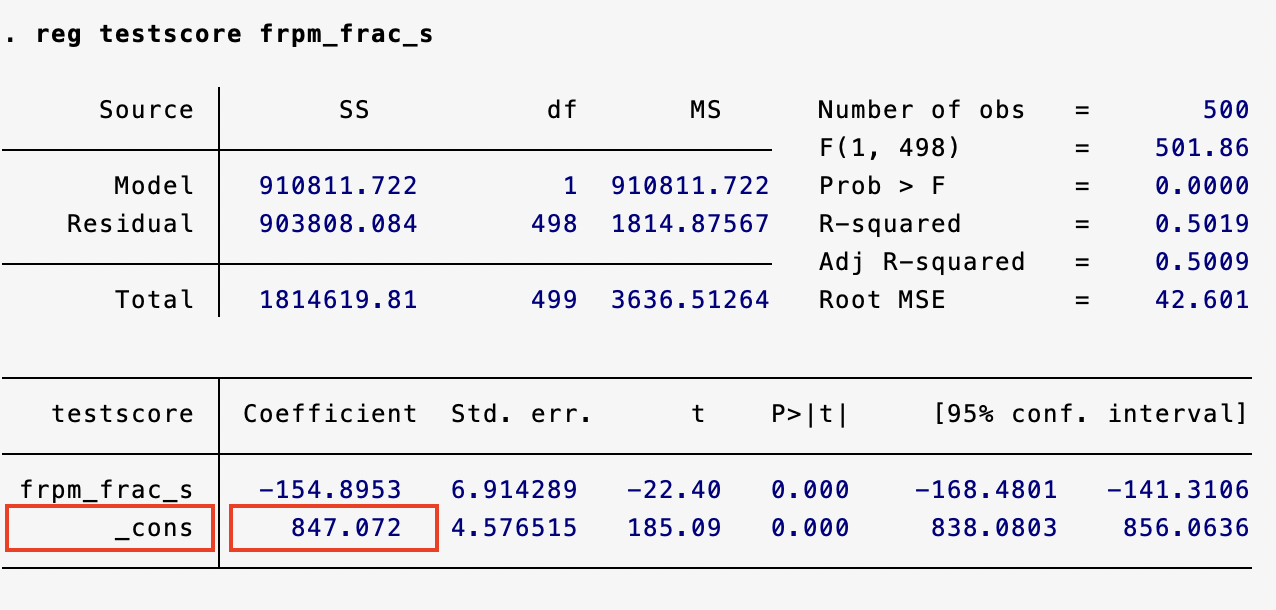
\includegraphics[scale=.4]{images/reg1.png}
\end{figure}
\end{column}
\end{columns}
\begin{equation*}
    Y_i = 847.072 + \hat{\beta}_1 X_i + \hat{u}_i
\end{equation*}
\end{frame}


\begin{frame}{Stata Application}
 \begin{columns}
\begin{column}{0.3\textwidth}
\begin{itemize}
    \item The estimate of the regression slope, $\hat{\beta}_1$ is equal to -154.8953
    \item An 10\%-pt increase in the share of subsidized meals is associated with a 15.49 decrease in the average level of test scores
    \item This represents a 25.69\% reduction in the standard deviation of test scores
\end{itemize}
\end{column}
\begin{column}{0.6\textwidth}
\begin{figure}
  \centering
         \vspace{-5mm}
        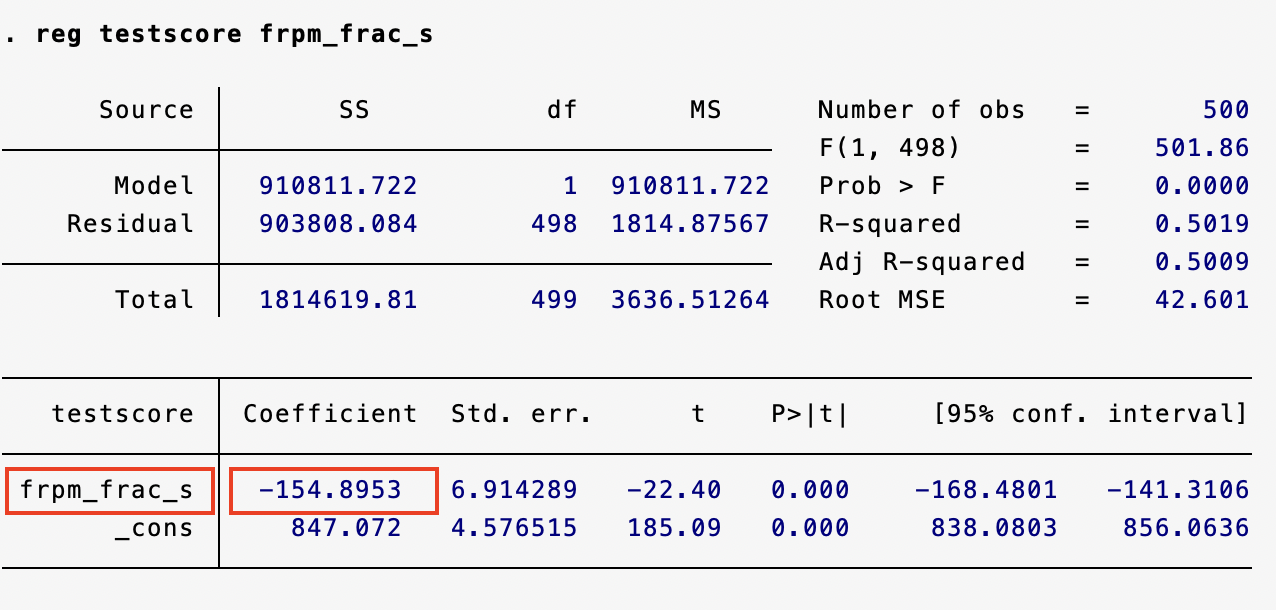
\includegraphics[scale=.4]{images/reg2.png}
\end{figure}
\end{column}
\end{columns}
\begin{equation*}
    Y_i = 847.02 -154.8953 X_i + \hat{u}_i
\end{equation*}
\end{frame}


\begin{frame}{Stata Application}
 \begin{columns}
\begin{column}{0.3\textwidth}
\begin{itemize}
    \item The estimate of the intercept, $\hat{\beta}_0$ is significantly different from 0.
    \item $\mid t_{\hat{\beta}_0} \mid = 185.09 >> 2.54 $ (or, alternatively, $p-value < .01$
    \item We reject $H_0: \beta_0 = 0 $  at the 1\% level
\end{itemize}
\end{column}
\begin{column}{0.6\textwidth}
\begin{figure}
  \centering
         \vspace{-5mm}
         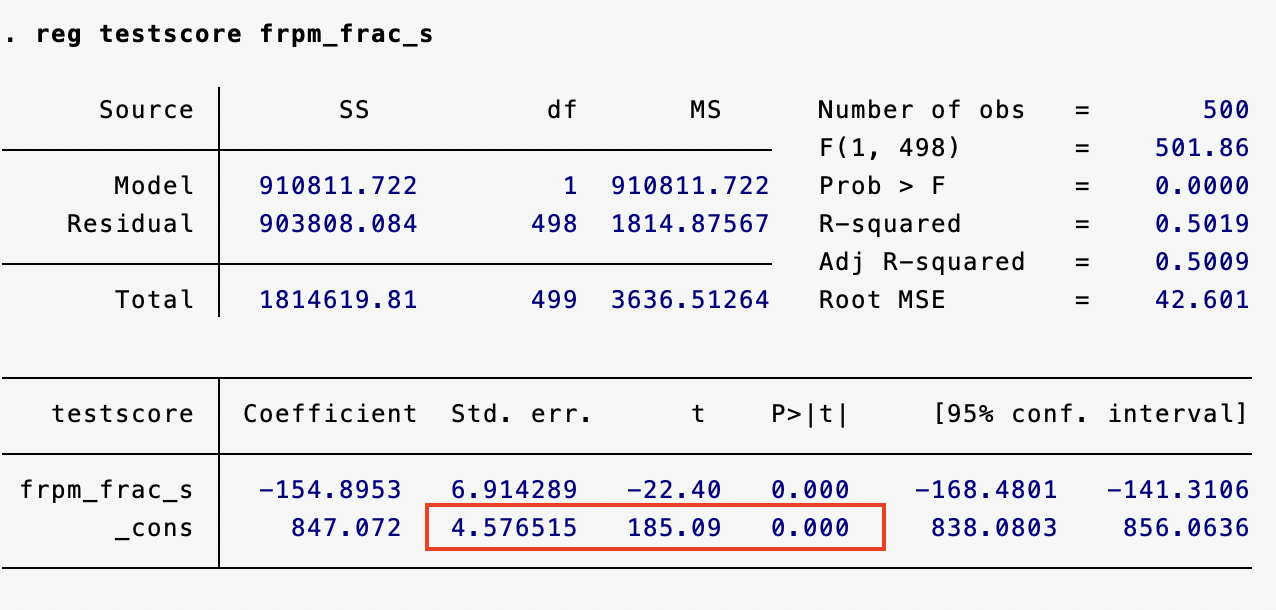
\includegraphics[scale=.4]{images/reg3.png}
\end{figure}
\end{column}
\end{columns}
\begin{center}
\begin{eqnarray*}
    &Y_i = &847.02 -154.8953 X_i + \hat{u}_i\\
    &  &[4.576] 
\end{eqnarray*}
\end{center}
\end{frame}


\begin{frame}{Stata Application}
 \begin{columns}
\begin{column}{0.3\textwidth}
\begin{itemize}
    \item The estimate of the regression slope, $\hat{\beta}_1$ is significantly different from 0.
    \item $\mid t_{\hat{\beta}_1} \mid = 22.4 >> 2.54 $ (or, alternatively, $p-value < .01$
    \item We reject $H_0: \beta_1 = 0 $ at the 1\% level
\end{itemize}
\end{column}
\begin{column}{0.6\textwidth}
\begin{figure}
  \centering
         \vspace{-5mm}
         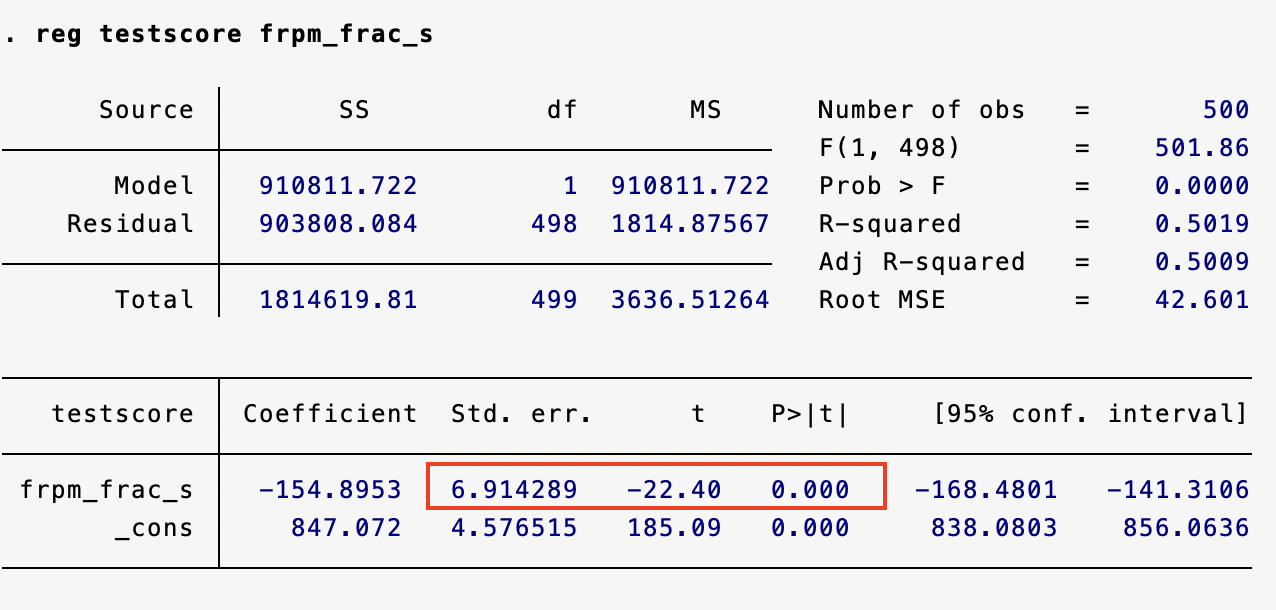
\includegraphics[scale=.4]{images/reg4.png}
\end{figure}
\end{column}
\end{columns}
\begin{center}
\begin{eqnarray*}
    Y_i = &847.02 &-154.8953 X_i + \hat{u}_i\\
      &[4.576] &~~~~[6.914]
\end{eqnarray*}
\end{center}
\end{frame}



\begin{frame}{Stata Application}
 \begin{columns}
\begin{column}{0.3\textwidth}
Recall that the CI defines
\begin{itemize}
    \item The set of points that cannot be rejected at the 5\% significance level;
    \item A set-valued function of the data (an interval that is a function of the data) that contains the true parameter value 95\% of the time in repeated samples.
    \end{itemize}
\end{column}
\begin{column}{0.6\textwidth}
\begin{figure}
  \centering
         \vspace{-5mm}
        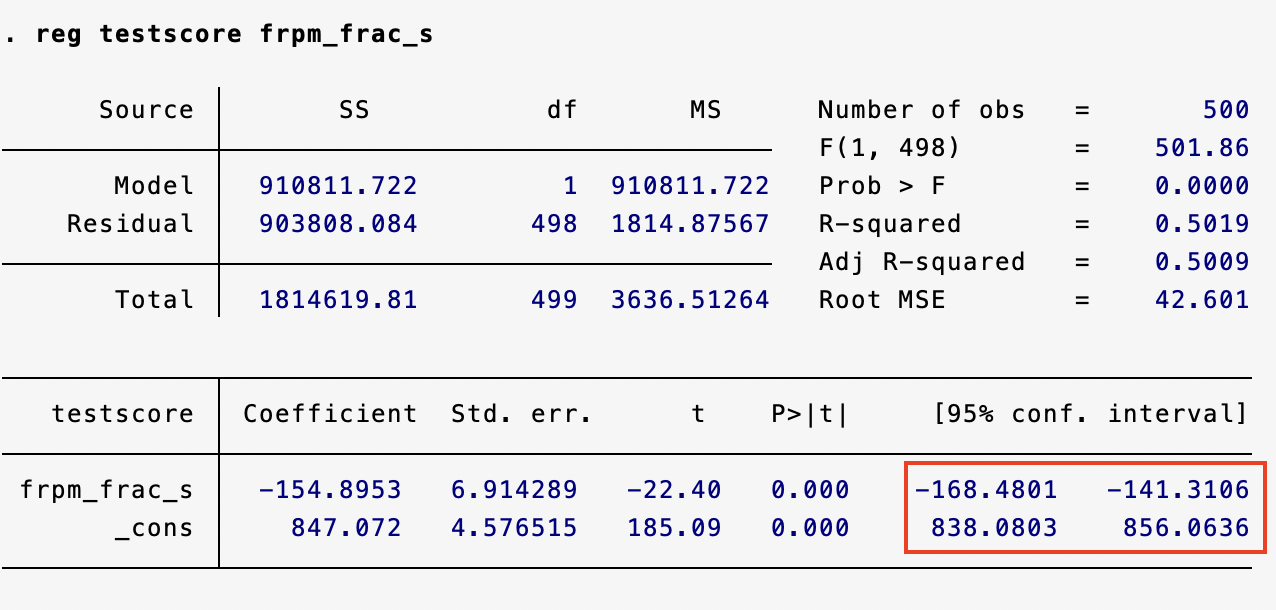
\includegraphics[scale=.4]{images/reg5.png}
\end{figure}
\end{column}
\end{columns}
\begin{center}
\begin{eqnarray*}
    &CI_{\beta_0} &= 847.072 + 1.96\pm 4.576 = [838.0803 ; 856.0636]\notin 0\\
    &CI_{\beta_1} &= -154.895 + 1.96\pm 6.914 = [ -168.4801 ; -141.3106]\notin 0
\end{eqnarray*}
\end{center}
\end{frame}


\begin{frame}{Stata Application}
 \begin{columns}
\begin{column}{0.3\textwidth}
Remember that
\begin{itemize}
    \item The SER measures the spread of the distribution of $u$ around the regression line in the units of the dependent variable.
    \item It is an estimator of the standard deviation of the regression error $u_i$.
\end{itemize}
\end{column}
\begin{column}{0.6\textwidth}
\begin{figure}
  \centering
        \vspace{-5mm}
        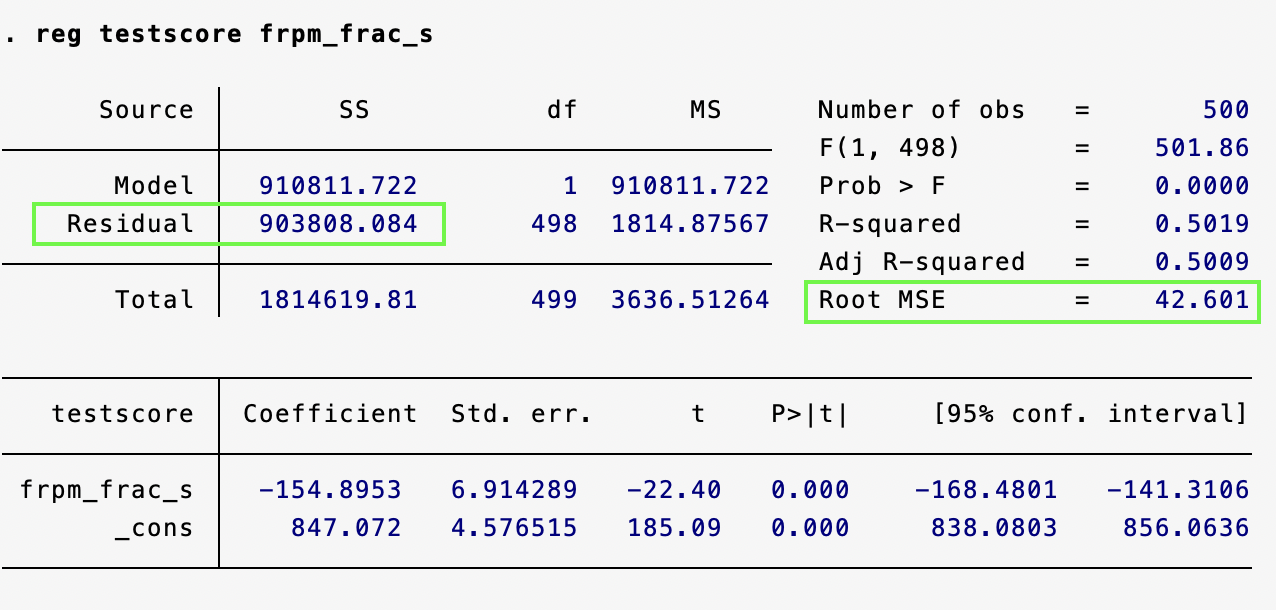
\includegraphics[scale=.4]{images/reg7.png}
\end{figure}
\end{column}
\end{columns}
\begin{center}
\begin{eqnarray*}
    SER = \sqrt{\frac{SSR}{n-2}}=\sqrt{\frac{\sum_{i=1}^n (\hat{u}_i-\overline{\hat{u}}_i)^2}{n-2}}=\sqrt{\frac{903808.084}{498}}\approx 42.601
\end{eqnarray*}
\end{center}
\end{frame}

\begin{frame}{Stata Application}
 \begin{columns}
\begin{column}{0.3\textwidth}
Remember that
\begin{itemize}
    \item The regression $R^2$ measures the fraction of the variance of Y that is explained by X
    \item It is unitless and ranges between zero (no fit) and one (perfect fit)
\end{itemize}
\end{column}
\begin{column}{0.6\textwidth}
\begin{figure}
  \centering
        \vspace{-5mm}
        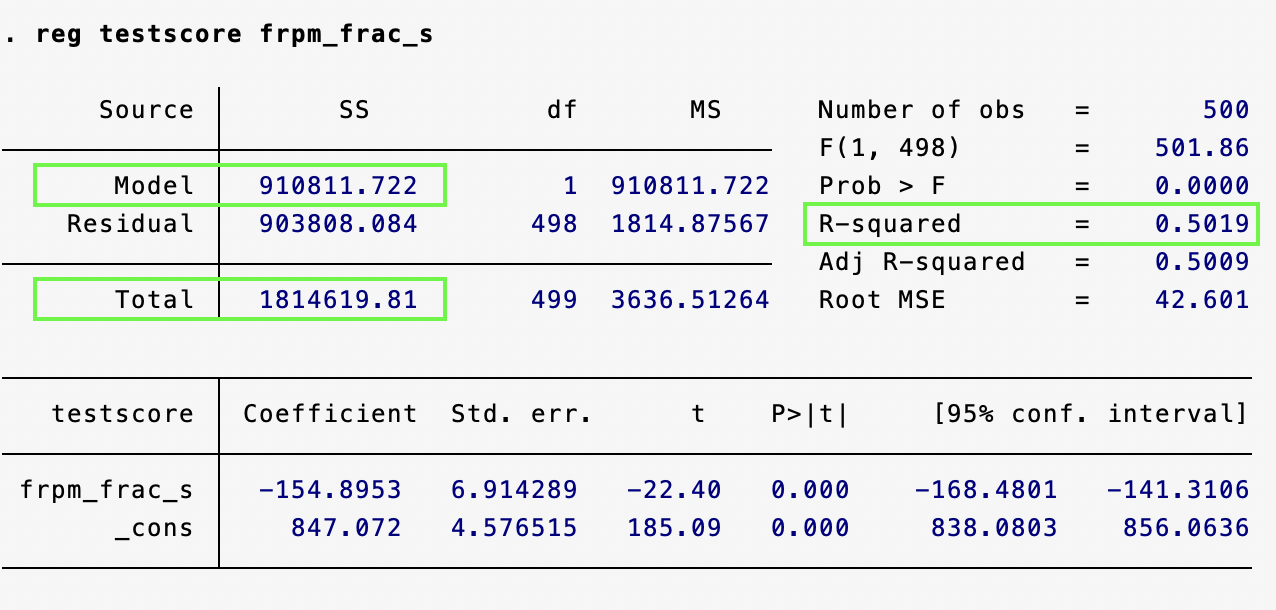
\includegraphics[scale=.4]{images/reg6.png}
\end{figure}
\end{column}
\end{columns}
\begin{center}
\begin{eqnarray*}
    &R^2 &= \frac{\text{explained sum of squares ($ESS$)}}{\text{total sum of squares ($TSS$)}} = \frac{\sum_{i=1}^n (\hat{Y}_i - \overline{Y})^2}{\sum_{i=1}^n (Y_i - \overline{Y})^2}=\frac{910811.722}{1814619.81}\approx  0.5019\\
\end{eqnarray*}
\end{center}
\end{frame}


\begin{frame}
\frametitle{Homoskedasticity vs. Heteroskedasticity}

\begin{itemize}
    \item In regression analysis, we often make an important assumption about the variance of the error term, $u$, known as \textbf{homoskedasticity}.
    \item Homoskedasticity implies that the variance of the error term is constant for all observations.
    \item However, in most cases, this assumption may not hold, leading to \textbf{heteroskedasticity}, where the variance of $u$ varies across observations.
\end{itemize}
\begin{block}{Homoskedasticity vs. Heteroskedasticity}
For homoskedastic data, we assume:
\[
\text{var}(u_i \mid X) = \sigma^2 \quad \text{for all } i
\]

For heteroskedastic data, the variance of $u_i$ is not constant:
\[
\text{var}(u_i \mid X) = \sigma_i^2 \quad \text{for each } i
\]
\end{block}

\end{frame}


\begin{frame}{Graphical Illustration}
 \begin{columns}
\begin{column}{0.35\textwidth}
    \begin{itemize}
    \item Understanding \textbf{homoskedasticity} and heteroskedasticity is crucial in regression analysis.
    \item \textbf{Homoskedasticity} assumes constant error variance, while heteroskedasticity implies varying error variance.
    \item To account for heteroskedasticity, robust standard errors can be used to obtain valid inferences.
    \end{itemize}
\end{column}
\begin{column}{0.7\textwidth}
\begin{figure}
  \centering
         \vspace{-5mm}
        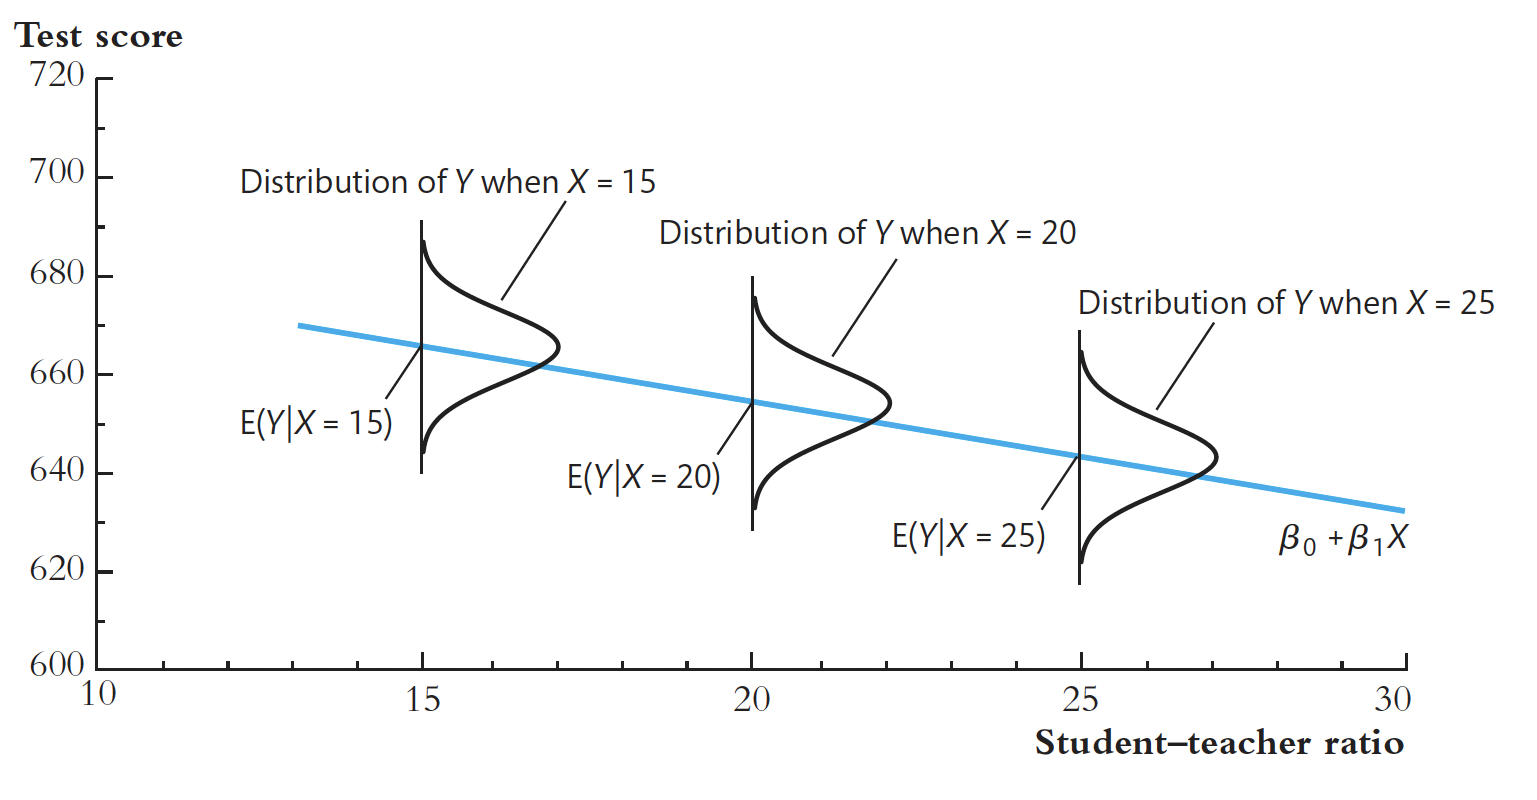
\includegraphics[scale=.35]{images/homoskedastic.png}
\end{figure}
\end{column}
\end{columns}
\end{frame}

\begin{frame}{Graphical Illustration}
 \begin{columns}
\begin{column}{0.35\textwidth}
    \begin{itemize}
    \item Understanding homoskedasticity and \textbf{heteroskedasticity} is crucial in regression analysis.
    \item Homoskedasticity assumes constant error variance, while \textbf{heteroskedasticity} implies varying error variance.
    \item To account for \textbf{heteroskedasticity}, robust standard errors can be used to obtain valid inferences.
    \end{itemize}
\end{column}
\begin{column}{0.7\textwidth}
\begin{figure}
  \centering
         \vspace{-5mm}
        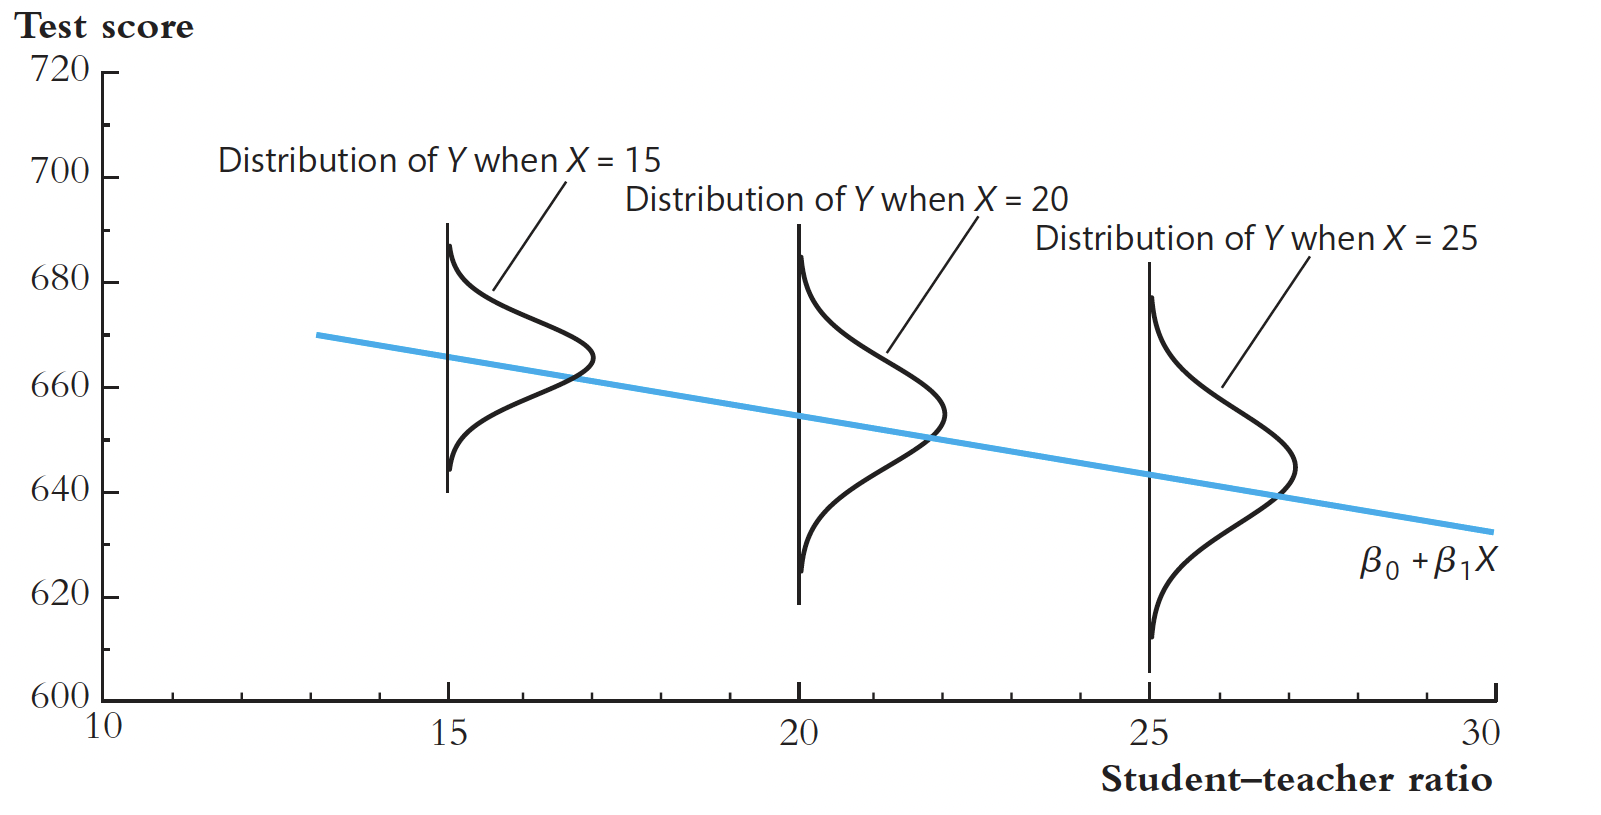
\includegraphics[scale=.35]{images/heteroskedastic.png}
\end{figure}
\end{column}
\end{columns}
\end{frame}

\begin{frame}{$var[\hat{\beta}_1]$ with robust standard errors}
\begin{eqnarray*}
& var(\hat{\beta}_1 \mid X) =  var(\hat{\beta}_1 - \beta_1 \mid X) &= var\left[\frac{\sum_{i=1}^n (X_i - \overline{X})u_i}{\sum_{i=1}^n (X_i - \overline{X})^2}\Bigg|X\right]\\
& &= var\left[\frac{\sum_{i=1}^n (X_i - \overline{X})u_i}{TSS_X}\Bigg|X\right]\\
& &= \frac{1}{TSS_X^2}var\left[\sum_{i=1}^n (X_i - \overline{X})u_i\bigg|X\right]\\
& &= \frac{\sum_{i=1}^n (X_i - \overline{X})^2 var(u_i\mid X)}{TSS_X^2}\\
%& &= \frac{\frac{1}{n}\sum_{i=1}^n (X_i - \overline{X})^2 var(u_i\mid X)}{ \frac{1}{n} TSS_X^2}\\
& &= \frac{\frac{1}{n}\sum_{i=1}^n (X_i - \overline{X})^2 var(u_i\mid X)}{ \frac{n-1}{n} s_X^2}\\
\end{eqnarray*}
\end{frame}


\begin{frame}{$var[\hat{\beta}_1]$ with robust standard errors}
So, when $n$ is large $var(\hat{\beta}_1)$ converges toward 
\begin{eqnarray*}
     \sigma^2_{\hat{\beta}_1} =\frac{\sum_{i=1}^n (X_i - \mu_X)^2 var(u_i\mid X)}{n \sigma_X^2}
\end{eqnarray*}
and $\hat{\beta}_1 \sim \mathcal{N}(\beta_1; \frac{\sigma_\nu^2}{n \sigma_X^2})$ where $\nu=(X_i - \mu_X)u_i$\\\vspace{.5cm}
The (robust) natural estimator of $\sigma^2_{\hat{\beta}_1}$ follows:
\begin{eqnarray*}
     \hat{\sigma}^2_{\hat{\beta}_1} =\frac{1}{n}\frac{\frac{1}{n-2}\sum_{i=1}^n (X_i - \overline{X})^2 \hat{u}_i^2}{\left[\frac{1}{n}\sum_{i=1}^n (X_i - \overline{X})\right]^2}
\end{eqnarray*}\\\vspace{.5cm}
(Heteroskedasticity-)Robust standard errors (or Eicker–Huber–White standard errors) are then $SE(\hat{\beta_1})=\sqrt{\hat{\sigma}^2_{\hat{\beta}_1}}$
\end{frame}


\begin{frame}{In practice}
 \begin{columns}
\begin{column}{0.35\textwidth}
    \begin{itemize}
    \item If the errors are either homoskedastic or heteroskedastic and you use heteroskedastic-robust standard errors, you are OK
    \item If the errors are heteroskedastic and you use the homoskedasticity-only formula for standard errors, your standard errors will be wrong
    \end{itemize}
\end{column}
\begin{column}{0.6\textwidth}
\begin{figure}
  \centering
         \vspace{-5mm}
        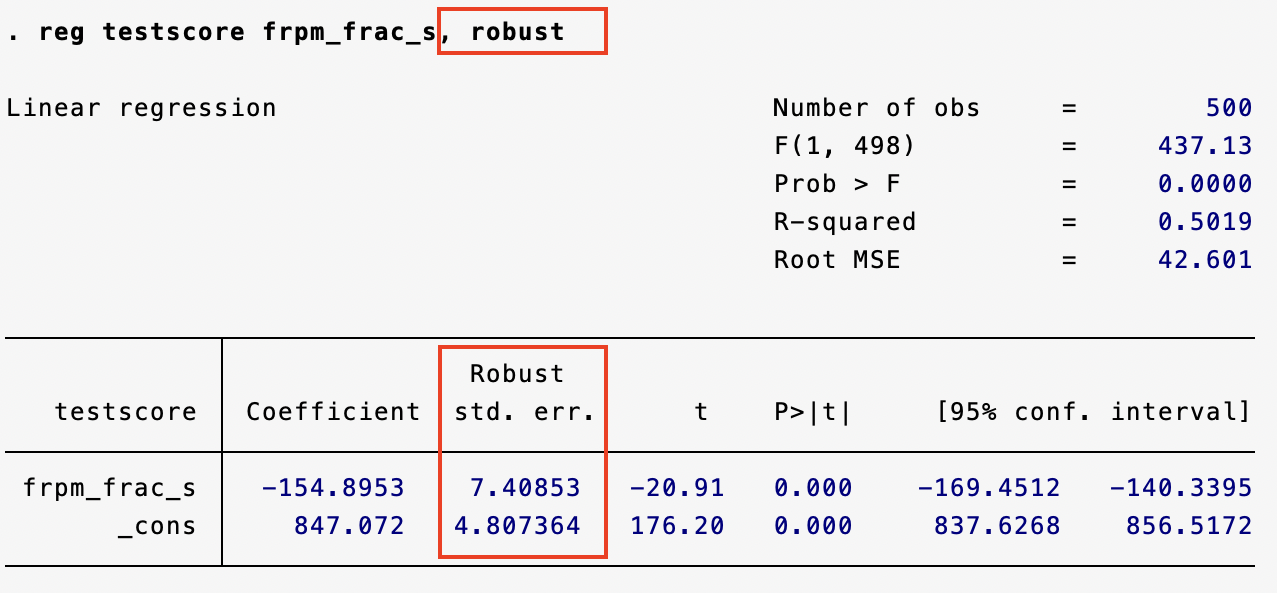
\includegraphics[scale=.4]{images/regrobust.png}
\end{figure}
\end{column}
\end{columns}
    \begin{itemize}
    \item The homoskedasticity-only estimator of the variance of $\hat{\beta}_1$ is inconsistent if there is heteroskedasticity.
    \end{itemize}
\end{frame}


\begin{frame}{The Theoretical Foundations of OLS}

Let us consider a linear regression model:

\[
Y_i = \beta_0 + \beta_1 X_{i}  + u_i
\]

Subject to the following assumptions:

\begin{enumerate}
    \item Zero Conditional Mean: The errors $u_i$ have a conditional mean of zero given the values of the independent variables, i.e., $\mathbb{E}(u_i|X_{i}) = 0$ for all $i$.

    \item Random Draws: observations $(Y_i;X_i)$ are randomly drawn from the same population distribution, i.e., they are i.i.d. for all $i$.
    
    \item Large outliers are rare: $\mathbb{E}(Y^4)<\infty$ and $\mathbb{E}(X^4)<\infty$
    
    \item Homoskedasticity: The errors have constant variance, i.e., $\text{Var}(u_i) = \sigma_u^2$ for all $i$.
    
    \item u is normally distributed: $u\sim\mathcal{N}(0;\sigma_u^2)$.
\end{enumerate}

\begin{exampleblock}{Gauss-Markov Theorem}
Under assumptions 1-4, the OLS estimators are Best Linear Unbiased Estimators (BLUE).
\end{exampleblock}
\end{frame}

\begin{frame}{The Gauss-Markov Theorem}
\begin{itemize}
    \item The OLS estimator $\hat{\beta}_1$ is a linear estimator, that is, it can be written as a linear function of $Y_1, ..., Y_n$:
    \begin{eqnarray*}
        &\hat{\beta}_1-\beta_1 = \frac{\sum_{i=1}^n (X_i - \overline{X})u_i}{\sum_{i=1}^n(X_i - \overline{X})^2}\equiv w^{OLS}_iu_i\\
        \text{where} &w^{OLS}_i=\frac{\sum_{i=1}^n (X_i - \overline{X})}{\sum_{i=1}^n(X_i - \overline{X})^2}
    \end{eqnarray*}
    \item The Gauss-Markov theorem states that among all possible choices of $\{w_i\}$ the OLS weights $w^{OLS}_i$ yield the smallest $var(\hat{\beta}_1)$.
    \item Under assumptions 1-5, the ordinary least squares (OLS) estimators $\hat{\beta}_0$ and $\hat{\beta}_1$  have the minimum variance among all (linear and non-linear) unbiased estimators
\end{itemize}
\end{frame}

\begin{frame}{The Gauss-Markov Theorem: Limits}
The Gauss-Markov Theorem is a crucial justification for using OLS in many regression analyses, but it is very restrictive and, therefore, has serious practical limitations.
\begin{itemize}
    \item The result is only for linear estimators –- only a small subset of estimators
    \item The condition of homoskedasticity often doesn’t hold (homoskedasticity is a special case)
    \item When estimating the population mean, if there are significant outliers, the median is preferred over the mean because it's less sensitive and has lower variance. Similarly, in regression, OLS estimators can also be sensitive to outliers. In such cases, other estimators like the Least Absolute Deviations (LAD) estimator may be more efficient:
    \begin{eqnarray*}
        \min_{\hat{\beta}_0;\hat{\beta}_1}\sum_{i=1}^n \mid Y_i - \beta_0 - \beta_1 X_i \mid 
    \end{eqnarray*}
\end{itemize}
\end{frame}


\begin{frame}{Back to the original question}
Suppose schools receive extra transfers from the central government so the share of subsidized school meals increases by 10\%-pt. What is the effect of this policy intervention (“treatment”) on test scores? 
\begin{itemize}
    \item This question requires an estimate of the causal effect on test scores of a change in the share of subsidized meals. Does our regression analysis using the California data set provide a compelling estimate of this causal effect?
    \item Not really – districts with a low share of subsidized meals tend to be ones with lots of other resources and higher income families, which provide kids with more learning opportunities outside school…this suggests that $corr(u_i; X_i)>0$ (that is, $\mathbb{E}(u_i\mid X_i)\neq 0$).
    \item It seems that we have omitted some factors, or variables, from our analysis, and this has biased our results…
\end{itemize}
\end{frame}


\begin{frame}[allowframebreaks]{Material}
\begin{itemize}
    \item[--] \textbf{Textbooks:}
    \begin{itemize}
        \item Introduction to Econometrics, 4th Edition, Global Edition, by Stock and Watson -- Chapter 5
    \end{itemize}
\end{itemize}
\end{frame}


\end{document}
